% --------------------------------------------------------------------------- %
% --------------------------------------------------------------------------- %
\chapter{Results}
\label {ch:results}
% --------------------------------------------------------------------------- %
% --------------------------------------------------------------------------- %
The results of this search are shown in the next section.
The \MET\ distribution is shown for each of the five signal regions,
along with a yield table that shows the predictions for each of the three major backgrounds binned in \MET\ and the observed data yield.
No significant excesses were seen with respect to the standard model prediction.
In the final sections of this chapter,
the results are interpreted in the context of the signal model described in section~\ref{sec:signalmodel}.

\section{Results in Signal Region A}
The results for signal region A are shown separately in the b-veto region, and in the signal region when requiring at least 1 b-tagged jet.
The uncertainties in the tables and plots include the systematic uncertainties described in chapter~\ref{ch:bkgd}.

\begin{table}[htb]
  \scriptsize
  \begin{center}
    \caption{\label{tab:results_bveto_SRA} 
      Results are shown for signal region A when requiring a b-veto.
      Systematic uncertainties for each region are included in the total uncertainty. 
    }
    \scalebox{0.8}{
      \begin{tabular}{l|c|c|c|c|c|c}
        \hline
        \hline
        $\mathrm{E_{T}^{miss} [GeV]}$ &0 - 50 & 50 - 100 & 100 - 150 & 150 - 225 & 225 - 300 & $\geq$ 300 \\
        \hline 
        Z+jets&  1333.1 $\pm$ 62.0 &  314.4 $\pm$ 24.3 &  24.3 $\pm$ 4.3 &  4.6 $\pm$ 0.6 &  1.5 $\pm$ 0.4 &  1.1 $\pm$ 0.5 \\ 
        FS bkg&  5.3$^{+ 3.6}_{- 2.3}$ &  9.5$^{+ 4.3}_{- 3.1}$ &  3.2$^{+ 3.1}_{- 1.7}$ &  3.2$^{+ 3.1}_{- 1.7}$ &  1.1$^{+ 2.4}_{- 0.9}$ &  0.0$^{+ 1.2}_{- 0.0}$ \\ 
        Other SM&  1.7 $\pm$ 0.8 &  2.2 $\pm$ 1.1 &  1.6 $\pm$ 0.8 &  1.3 $\pm$ 0.6 &  0.8 $\pm$ 0.4 &  1.0 $\pm$ 0.5 \\ 
        \hline 
        total BG&  1340.0$^{+ 62.1}_{- 62.1}$ &  326.1$^{+ 24.7}_{- 24.6}$ &  29.1$^{+ 5.3}_{- 4.7}$ &  9.1$^{+ 3.2}_{- 1.9}$ &  3.4$^{+ 2.5}_{- 1.0}$ &  2.1$^{+ 1.4}_{- 0.7}$ \\ 
        \hline 
        Data&  1340 &  332 &  28 &  7 &  6 &  6 \\ 
        \hline
        \hline
      \end{tabular}
    }
  \end{center}
\end{table}


\begin{table}[htb]
  \scriptsize
  \begin{center}
    \caption{\label{tab:results_withb_SRA} 
      Results are shown for signal region A where at least 1 b-tagged jet is required.
      Systematic uncertainties for each region are included in the total uncertainty. 
    }
    \scalebox{0.8}{
      \begin{tabular}{l|c|c|c|c|c|c}
        \hline
        \hline
        $\mathrm{E_{T}^{miss} [GeV]}$ &0 - 50 & 50 - 100 & 100 - 150 & 150 - 225 & 225 - 300 & $\geq$ 300 \\
        \hline 
        Z+jets&  182.6 $\pm$ 24.1 &  53.0 $\pm$ 11.4 &  4.5 $\pm$ 0.9 &  1.4 $\pm$ 0.4 &  0.7 $\pm$ 0.3 &  0.2 $\pm$ 0.2 \\ 
        FS bkg&  5.3$^{+ 3.6}_{- 2.3}$ &  12.6$^{+ 4.8}_{- 3.6}$ &  9.5$^{+ 4.3}_{- 3.1}$ &  5.3$^{+ 3.6}_{- 2.3}$ &  5.3$^{+ 3.6}_{- 2.3}$ &  1.1$^{+ 2.4}_{- 0.9}$ \\ 
        Other SM&  0.2 $\pm$ 0.1 &  0.3 $\pm$ 0.1 &  0.3 $\pm$ 0.1 &  0.2 $\pm$ 0.1 &  0.1 $\pm$ 0.1 &  0.2 $\pm$ 0.1 \\ 
        \hline 
        total BG&  188.0$^{+ 24.4}_{- 24.2}$ &  65.9$^{+ 12.4}_{- 12.0}$ &  14.3$^{+ 4.4}_{- 3.2}$ &  6.9$^{+ 3.6}_{- 2.3}$ &  6.1$^{+ 3.6}_{- 2.3}$ &  1.5$^{+ 2.4}_{- 0.9}$ \\ 
        \hline 
        Data&  188 &  68 &  21 &  6 &  1 &  3 \\ 
        \hline
        \hline
      \end{tabular}
    }
  \end{center}
\end{table}

\begin{figure}[!ht]
  \begin{center}
    \begin{tabular}{cc}
      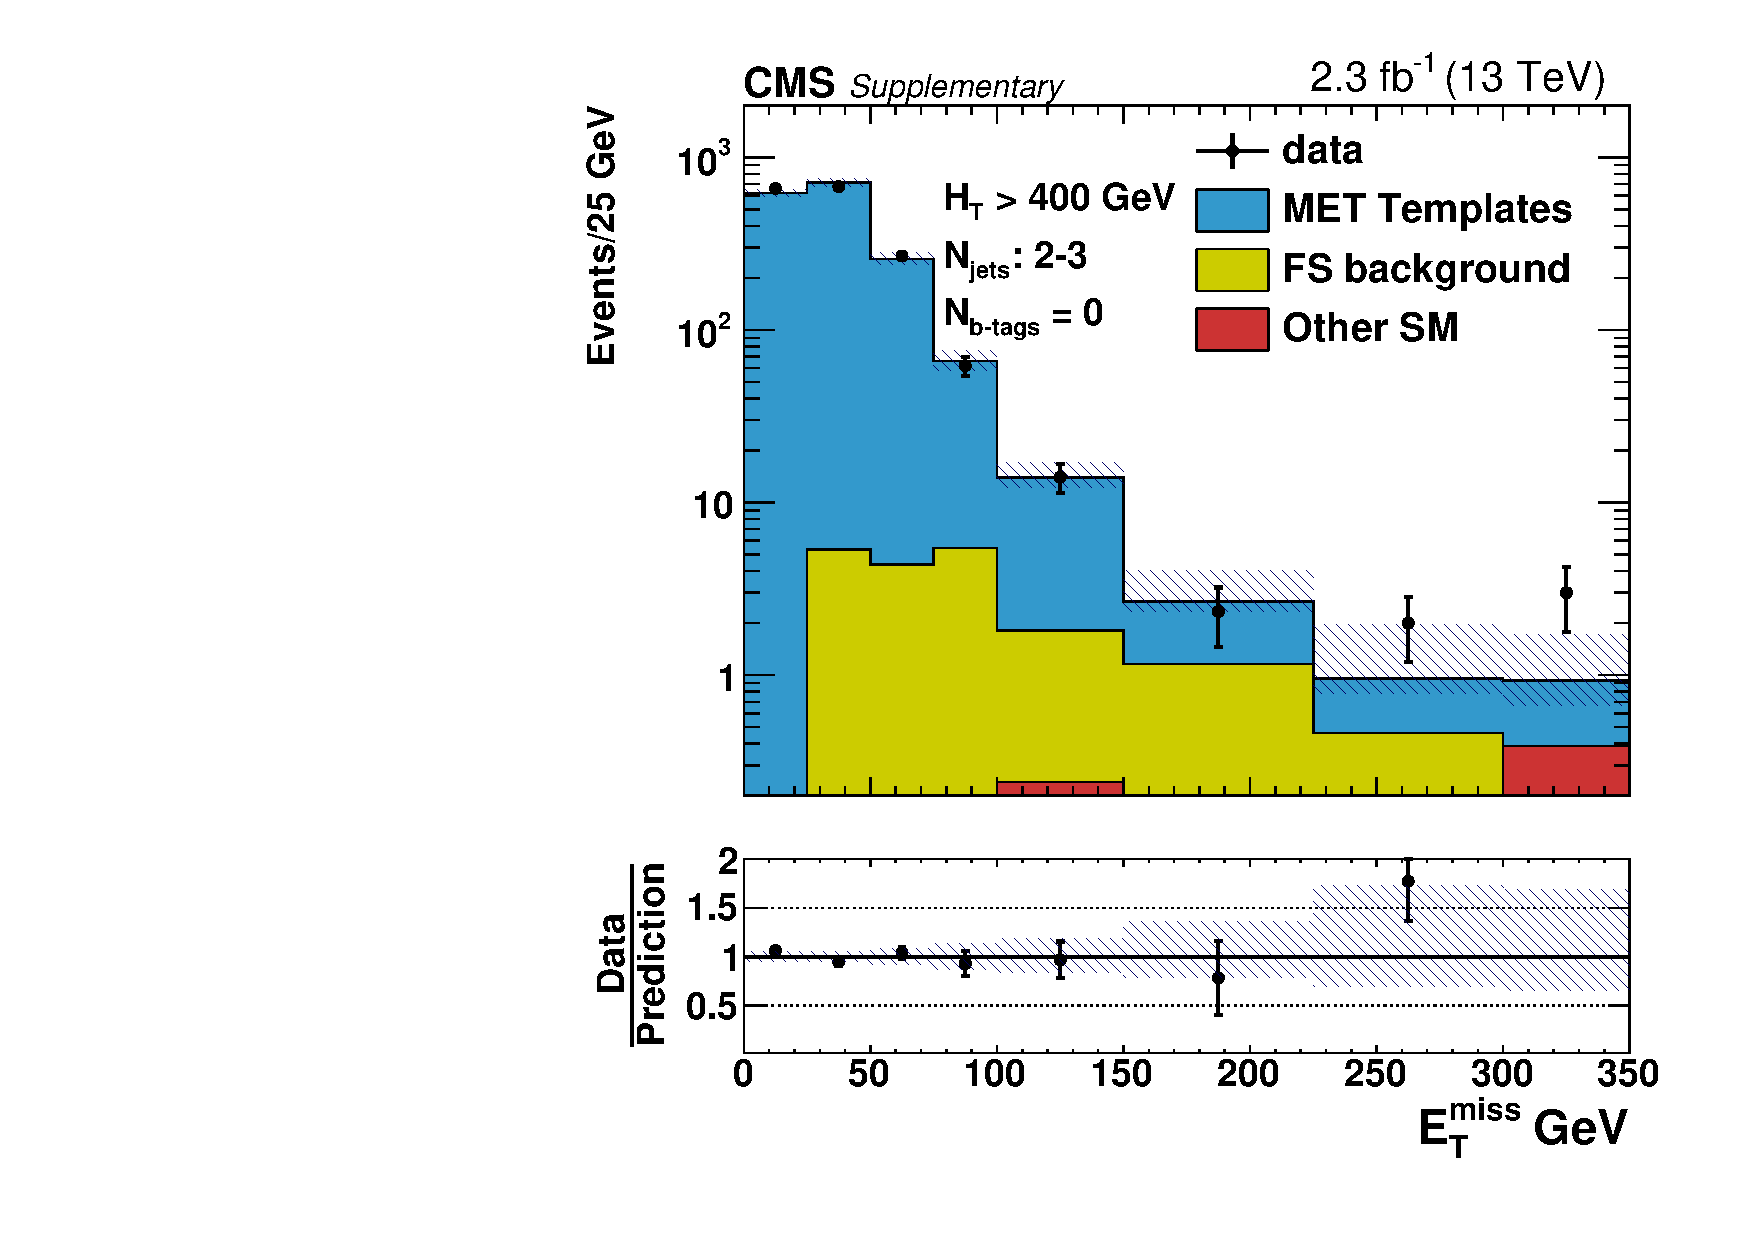
\includegraphics[width=0.4\textwidth]{results/figs/SRA_bveto_MET_yield_hist.pdf} &
      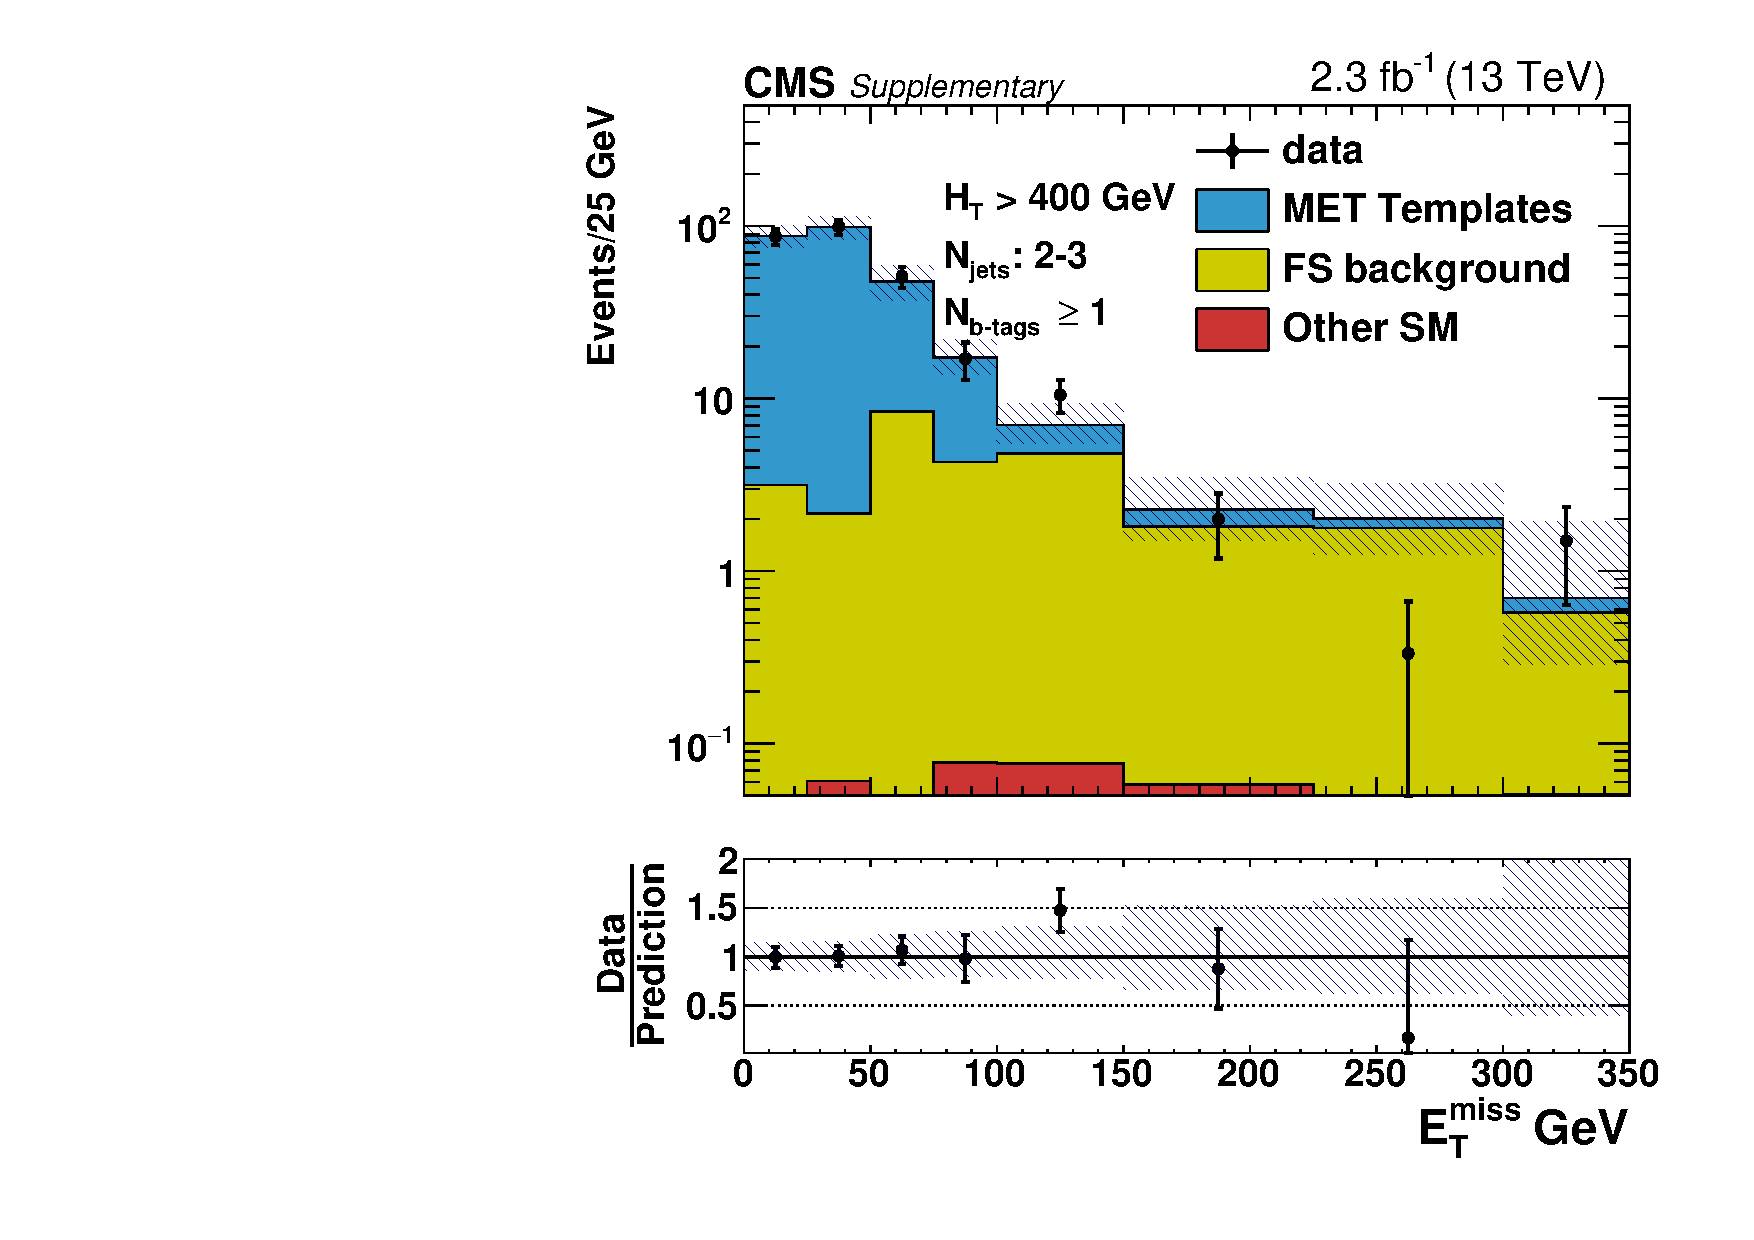
\includegraphics[width=0.4\textwidth]{results/figs/SRA_withb_MET_yield_hist.pdf} \\
    \end{tabular}
    \caption{
      The \MET\ distribution is shown for data vs. the data-driven predictions in signal region B.
      The left plot shows the prediction when requiring N$\mathrm{_{b-jets}} =$ 0, and the right plot shows the prediction when requiring N$\mathrm{_{b-jets}} \geq$ 1.
      The dashed line in the plot represents the full uncertainty.
      See tables~\ref{tab:results_bveto_SRA}~and~\ref{tab:results_withb_SRA}~for yields.
      \label{fig:results_SRA}
    }
  \end{center}
\end{figure}

\clearpage

\section{Results in Signal Region B}

The results for signal region A are shown separately in the b-veto region, and in the signal region when requiring at least 1 b-tagged jet.
The uncertainties in the tables and plots include the systematic uncertainties described in chapter~\ref{ch:bkgd}.

\begin{table}[htb]
  \scriptsize
  \begin{center}
    \caption{
      \label{tab:results_bveto_SRB} 
      Results are shown for signal region B when requiring a b-veto.
      Systematic uncertainties for each region are included in the total uncertainty. 
    }
    \scalebox{0.8}{
      \begin{tabular}{l|c|c|c|c|c|c}
        \hline
        \hline
        $\mathrm{E_{T}^{miss} [GeV]}$ &0 - 50 & 50 - 100 & 100 - 150 & 150 - 225 & 225 - 300 & $\geq$ 300 \\
        \hline 
        Z+jets&  1907.2 $\pm$ 68.8 &  282.5 $\pm$ 16.4 &  10.0 $\pm$ 0.9 &  3.2 $\pm$ 0.6 &  0.3 $\pm$ 0.1 &  0.1 $\pm$ 0.1 \\ 
        FS bkg&  9.5$^{+ 4.3}_{- 3.1}$ &  22.1$^{+ 6.0}_{- 4.9}$ &  12.6$^{+ 4.8}_{- 3.6}$ &  4.2$^{+ 3.3}_{- 2.0}$ &  0.0$^{+ 1.2}_{- 0.0}$ &  1.1$^{+ 2.4}_{- 0.9}$ \\ 
        Other SM&  1.4 $\pm$ 0.6 &  2.0 $\pm$ 0.8 &  1.0 $\pm$ 0.4 &  0.8 $\pm$ 0.3 &  0.5 $\pm$ 0.2 &  0.3 $\pm$ 0.1 \\ 
        \hline 
        total BG&  1918.0$^{+ 68.9}_{- 68.9}$ &  306.6$^{+ 17.5}_{- 17.1}$ &  23.6$^{+ 4.9}_{- 3.7}$ &  8.2$^{+ 3.4}_{- 2.1}$ &  0.8$^{+ 1.2}_{- 0.2}$ &  1.5$^{+ 2.4}_{- 0.9}$ \\ 
        \hline 
        Data&  1918 &  275 &  20 &  10 &  2 &  0 \\ 
        \hline
        \hline
      \end{tabular}
    }
  \end{center}
\end{table}


\begin{table}[htb]
  \scriptsize
  \begin{center}
    \caption{\label{tab:results_withb_SRB} 
      Results are shown for signal region B when requiring at least 1 b-tagged jet.
      Systematic uncertainties for each region are included in the total uncertainty. 
    }
    \scalebox{0.8}{
      \begin{tabular}{l|c|c|c|c|c|c}
        \hline
        \hline
        $\mathrm{E_{T}^{miss} [GeV]}$ &0 - 50 & 50 - 100 & 100 - 150 & 150 - 225 & 225 - 300 & $\geq$ 300 \\
        \hline 
        Z+jets&  415.4 $\pm$ 34.9 &  73.3 $\pm$ 8.0 &  5.0 $\pm$ 0.9 &  1.6 $\pm$ 0.3 &  0.4 $\pm$ 0.3 &  0.3 $\pm$ 0.2 \\ 
        FS bkg&  50.4$^{+ 8.6}_{- 7.5}$ &  70.4$^{+ 10.1}_{- 9.0}$ &  38.9$^{+ 7.6}_{- 6.5}$ &  14.7$^{+ 5.1}_{- 3.9}$ &  0.0$^{+ 1.2}_{- 0.0}$ &  1.1$^{+ 2.4}_{- 0.9}$ \\ 
        Other SM&  1.2 $\pm$ 0.5 &  1.5 $\pm$ 0.7 &  0.8 $\pm$ 0.4 &  0.5 $\pm$ 0.2 &  0.2 $\pm$ 0.1 &  0.1 $\pm$ 0.1 \\ 
        \hline 
        total BG&  467.0$^{+ 35.9}_{- 35.7}$ &  145.2$^{+ 12.9}_{- 12.0}$ &  44.7$^{+ 7.7}_{- 6.6}$ &  16.8$^{+ 5.1}_{- 3.9}$ &  0.6$^{+ 1.2}_{- 0.3}$ &  1.5$^{+ 2.4}_{- 0.9}$ \\ 
        \hline 
        Data&  467 &  152 &  45 &  23 &  4 &  3 \\ 
        \hline
        \hline
      \end{tabular}
    }
  \end{center}
\end{table}

\begin{figure}[!ht]
\begin{center}
\begin{tabular}{cc}
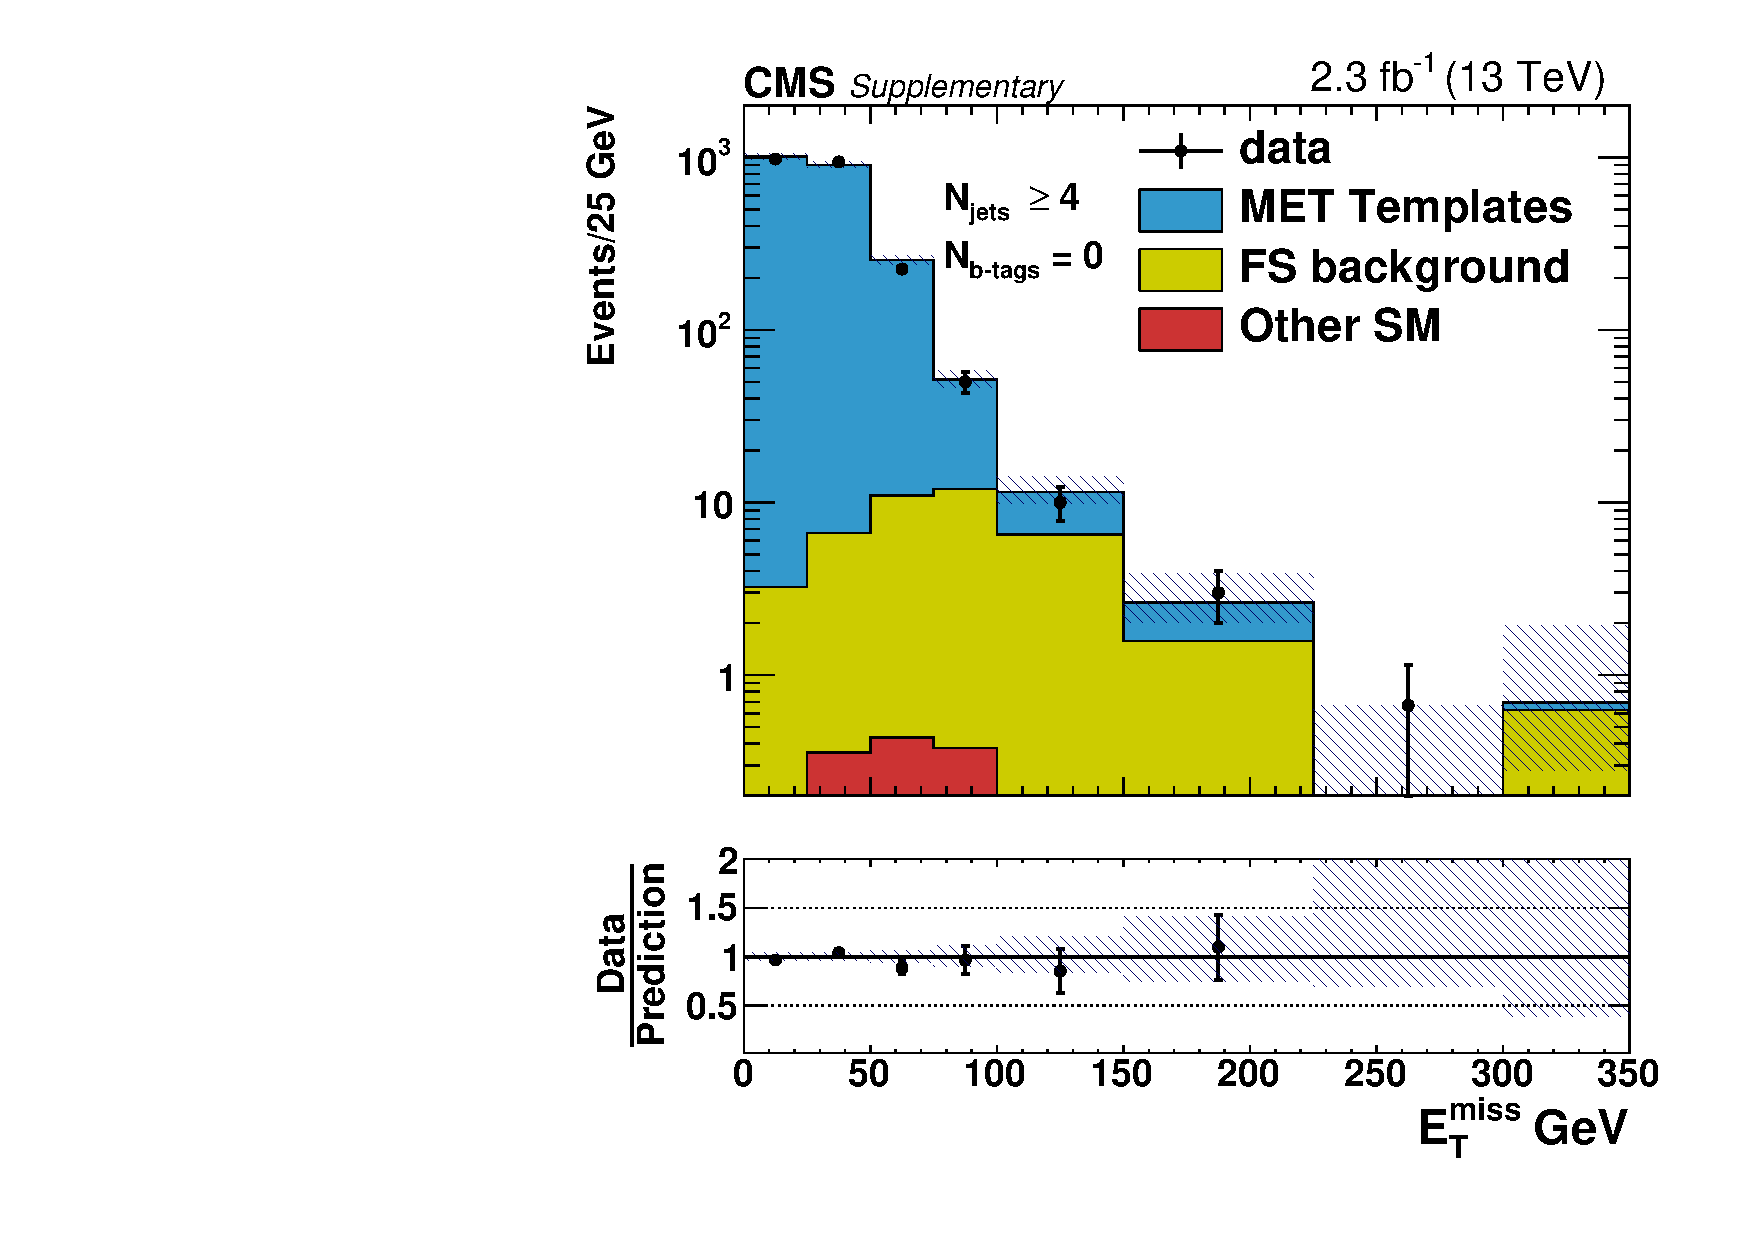
\includegraphics[width=0.4\textwidth]{results/figs/SRB_bveto_MET_yield_hist.pdf} &
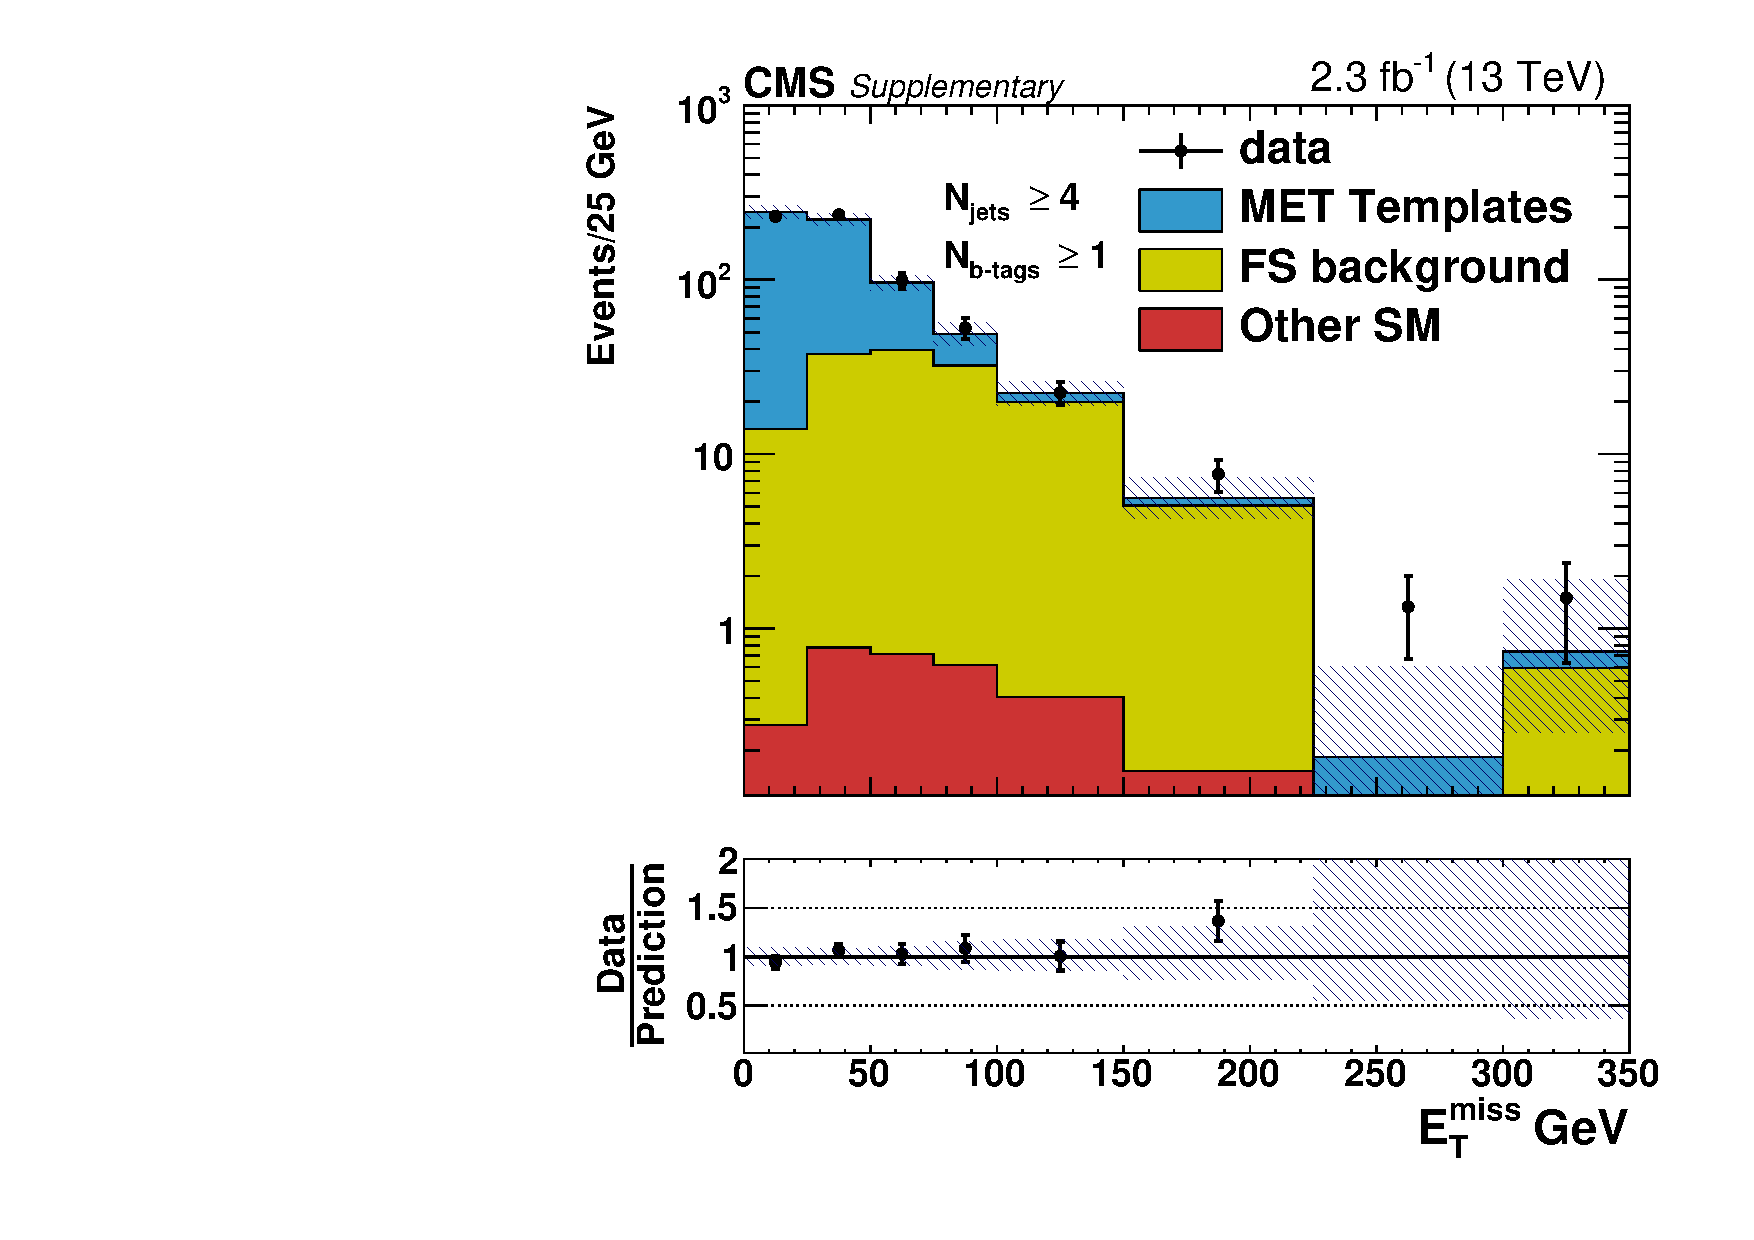
\includegraphics[width=0.4\textwidth]{results/figs/SRB_withb_MET_yield_hist.pdf} \\
\end{tabular}
\caption{
  \label{fig:results_SRB}
  The \MET\ distribution is shown for data vs. the data-driven predictions in signal region B.
  The left plot shows the prediction when requiring N$\mathrm{_{b-jets}} =$ 0, and the right plot shows the prediction when requiring N$\mathrm{_{b-jets}} \geq$ 1.
  The dashed line in the plot represents the full uncertainty.
  See tables~\ref{tab:results_bveto_SRB}~and~\ref{tab:results_withb_SRB}~for yields.
}
\end{center}
\end{figure}

\clearpage


\section{ATLAS-like signal regions}

The results for the ATLAS-like signal region in the on-Z search are shown in this section.
The signal regions defined as \MET\ $\geq$ 225 \gev.
The uncertainties in the tables and plots include the systematic uncertainties derived from the MC closure test.

\begin{table}[htb]
  \scriptsize
  \begin{center}
    \caption{\label{tab:results_SR_ATLAS} 
      Results are shown for the ATLAS signal region.
      Systematic uncertainties for each region are included in the total uncertainty. 
    }
    \scalebox{0.8}{
      \begin{tabular}{l|c|c|c|c|c}
        \hline
        \hline
        $\mathrm{E_{T}^{miss} [GeV]}$ &0 - 50 & 50 - 100 & 100 - 150 & 150 - 225 & $\geq$ 225 \\
        \hline 
        Z+jets&  1557.3 $\pm$ 56.6 &  386.2 $\pm$ 15.8 &  34.4 $\pm$ 5.0 &  8.1 $\pm$ 1.1 &  3.9 $\pm$ 0.7 \\ 
        FS bkg&  20.0$^{+ 5.8}_{- 4.6}$ &  21.0$^{+ 5.9}_{- 4.7}$ &  13.7$^{+ 5.0}_{- 3.8}$ &  13.7$^{+ 5.0}_{- 3.8}$ &  6.3$^{+ 3.8}_{- 2.5}$ \\ 
        Other SM&  2.8 $\pm$ 1.2 &  3.7 $\pm$ 1.6 &  2.3 $\pm$ 0.9 &  1.9 $\pm$ 0.8 &  2.1 $\pm$ 1.0 \\ 
        \hline 
        total BG&  1580.0$^{+ 57.0}_{- 56.8}$ &  410.9$^{+ 16.9}_{- 16.5}$ &  50.4$^{+ 7.1}_{- 6.3}$ &  23.6$^{+ 5.2}_{- 4.0}$ &  12.3$^{+ 4.0}_{- 2.8}$ \\ 
        \hline 
        Data&  1580 &  420 &  41 &  22 &  14 \\ 
        \hline
        \hline
      \end{tabular}
    }
  \end{center}
\end{table}


\begin{figure}[!ht]
\begin{center}
\begin{tabular}{cc}
%% 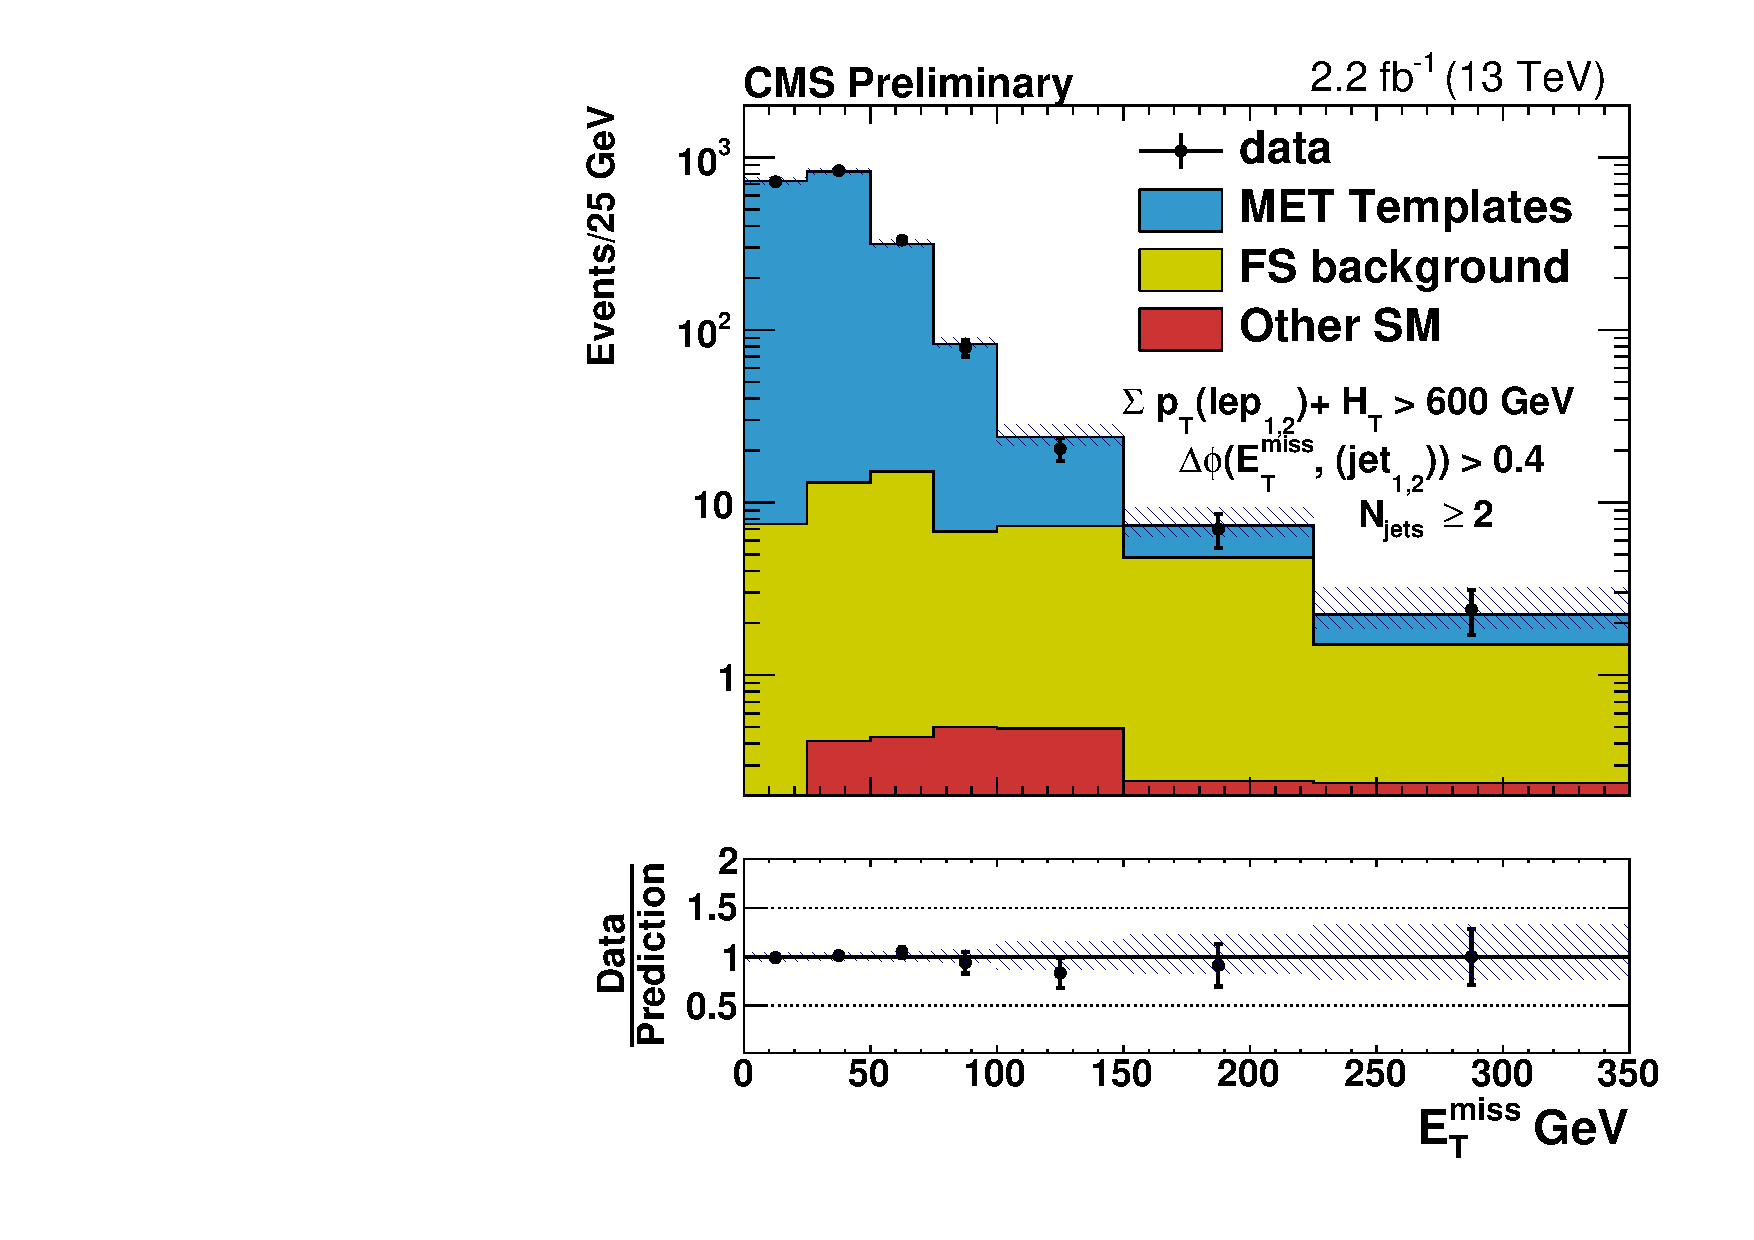
\includegraphics[width=0.8\textwidth]{results/figs/h_met_rawgt1jet_ll_signalregion_rawMET_loosephoton_SR_ATLAS_fsbkg_passtrig.pdf} \\
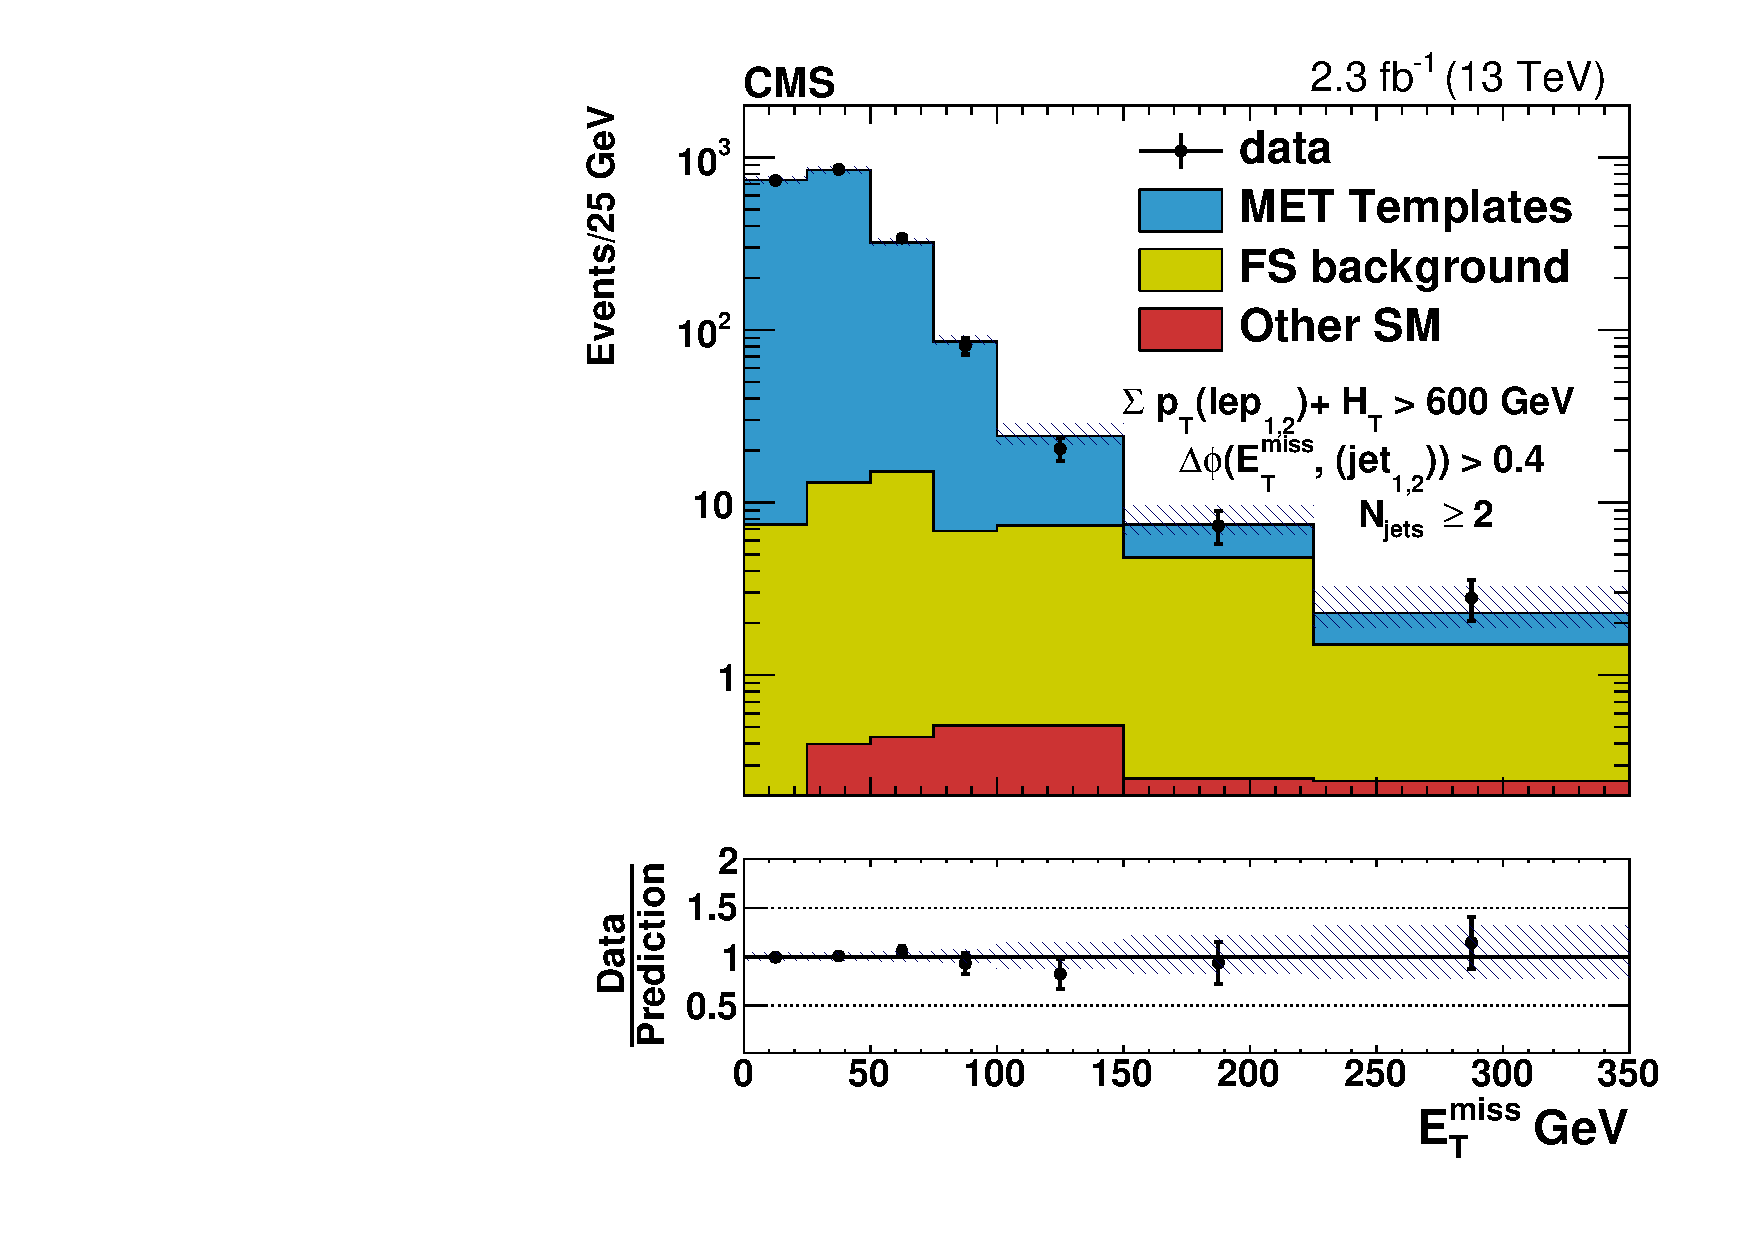
\includegraphics[width=0.8\textwidth]{results/figs/h_met_rawgt1jet_ll_signalregion_rawMET_SR_ATLAS_fsbkg_passtrig.pdf} \\
\end{tabular}
\caption{The \MET\ distribution is shown for data vs. the data-driven predictions in the ATLAS signal region.
See Tables~\ref{tab:results_bveto_SRA}~and~\ref{tab:results_SR_ATLAS}~for yields.
\label{fig:results_SR_ATLAS}
}
\end{center}
\end{figure}

\clearpage

\section{Systematic Uncertainties on Signal Model}

This section summarizes the systematic uncertainties assessed for the expected signal yields.
The sources of uncertainty are listed in table~\ref{tab:syst}, and they are described in detail in the section below.

\begin{table}[htb]
  \begin{center}
    \footnotesize
    \caption{
      \label{tab:syst}
      All systematic uncertainties of the expected signal yield are shown in this table.
    }
    \begin{tabular}{l|c}
      \hline
      \hline
      Source                     & Value (\%) \\
      \hline
      Luminosity                 & $\pm$2.7\%  \\
      PU reweighting             & $\pm$5\%    \\
      B-tag eff, heavy flavor    & $\pm$5\%    \\
      B-tag eff, light flavor    & $\pm$2\%    \\
      Lepton ID/Iso Efficiency   & $\pm$3\%    \\
      Fastsim Modeling           & $\pm$6\%    \\
      Lepton Trigger Efficiency  & $\pm$5\%    \\
      Jet Energy Scale           & $\pm$2-5\%  \\
      ISR Modeling               & $\pm$1\%    \\
      MC Statistics              & $\pm$5-20\% \\
      \hline
      Total uncertainty on signal& $\pm$13-24\% \\
      \hline
      \hline
    \end{tabular}
  \end{center}
\end{table}

\begin{description}

\item[Luminosity:] 
  Special runs are performed during the running of the LHC in order to assess the accuracy of the measured luminosity value.
  These runs are named Van Der Meer scans, after the physicist who first described this method~\cite{vdm}.
  The analysis of the Van Der Meer scans gives an uncertainty value of 2.7\%~\cite{lumi15up}.

\item[PU reweighting:] 
  The signal MC sample is reweighted such that the pileup distribution accurately reflects what is seen in data.
  When the nominal result is compared to what is seen when the pileup reweighting is not applied,
  differences of up to 5\% are seen for some mass points in the plane, so an uncertainty of 5\% is applied to account for these effects. 

\item[B-tagging Efficiency:] 
  Scale factors are applied in order to correct for the differences in efficiencies in data and MC when selecting b-tagged jets.
  The b-tagging scale factors are varied up and down using the uncertainties measured by the b-tagging POG at CMS~\cite{beff_2015}.  
  The scale factors are varied according to light-flavored and heavy-flavored jets separately. The uncertainty for heavy(light)-flavored jets is 5(2)\%.  

\item[Lepton ID/isolation Efficiency:] 
  Scale factors are applied in order to correct for the differences in efficiencies in data and MC when selecting applying lepton ID and isolation requirements.
  When the nominal result is compared to what is seen when the scale factors are not applied,
  differences of up to 3\% are seen for some mass points in the plane, so an uncertainty of 3\% is applied to account for these effects. 
  
\item[Modeling using FastSim:] 
  The signal MC is generated using Madgraph and Fastsim~\cite{fastsim},
  and scale factors are derived to correct for the differences in efficiency when comparing to Fullsim when selecting leptons.
  The scale factors are measured as a function of \pt\ and $\eta$ of the lepton.
  When the nominal result is compared to what is seen when the scale factors are not applied,
  differences of up to 6\% are seen for some mass points in the plane, so an uncertainty of 6\% is applied to account for these effects. 

\item[Lepton Trigger Efficiency:] 
  A flat scale factor is applied to the signal sample to account for the trigger efficiency using the efficiency measurements listed in table~\ref{tab:EffValues_Seperated}.
  An uncertainty of 5\% is assessed, which is meant to cover the difference in efficiency in the turn-on curve of each trigger.

\item[Jet Energy Scale:] 
  The jet energy scale is varied up and down within the uncertainties derived by the JETMET POG in CMS~\cite{cmsjetcal}\cite{jercworkgroup},
  and then these values are propagated through to all the objects used in the full analysis. 
  This gives a variation of up to 2(5)\% in expected signal yields in regions with \MET\ $<$ 300 ($>$ 300) \gev. 

\item[Modeling of Initial State Radiation:] 
  The signals for this analysis tend to have small ISR boost, so studies were performed in inclusive Z+jets and \ttbar\ regions to test the modeling of the initial state radiaion in MC.
  The results of this are shown in figure~\ref{fig:isrmodeling}, and scale factors were derived as a function of ISR \pt\ and used to derive an uncertainty of 1\% due to this effect.

\item[MC Statistics:] 
  The MC statistical uncertainty is taken into account, and after applying the signal selection less signal events are seen for lower values of \MET, and more events at high \MET.
  It varies from 5-20\% depending on the signal region and the point in the scan.

\end{description}

\begin{figure}[!ht]
\begin{center}
\begin{tabular}{cc}
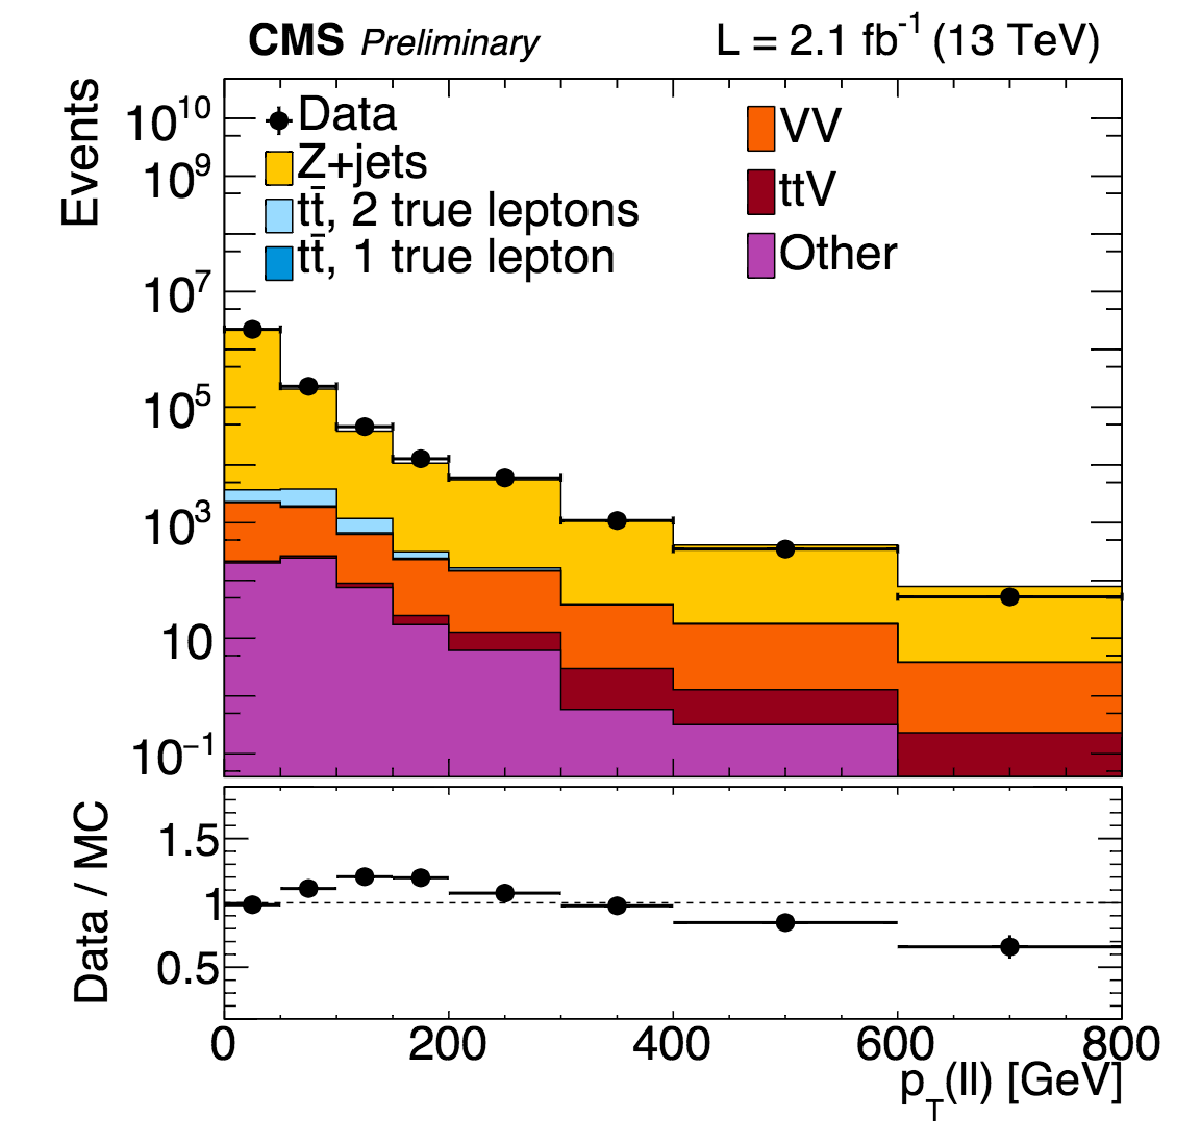
\includegraphics[width=0.4\textwidth]{results/figs/CMS-PAS-SUS-15-007_Figure_010-a.pdf} &
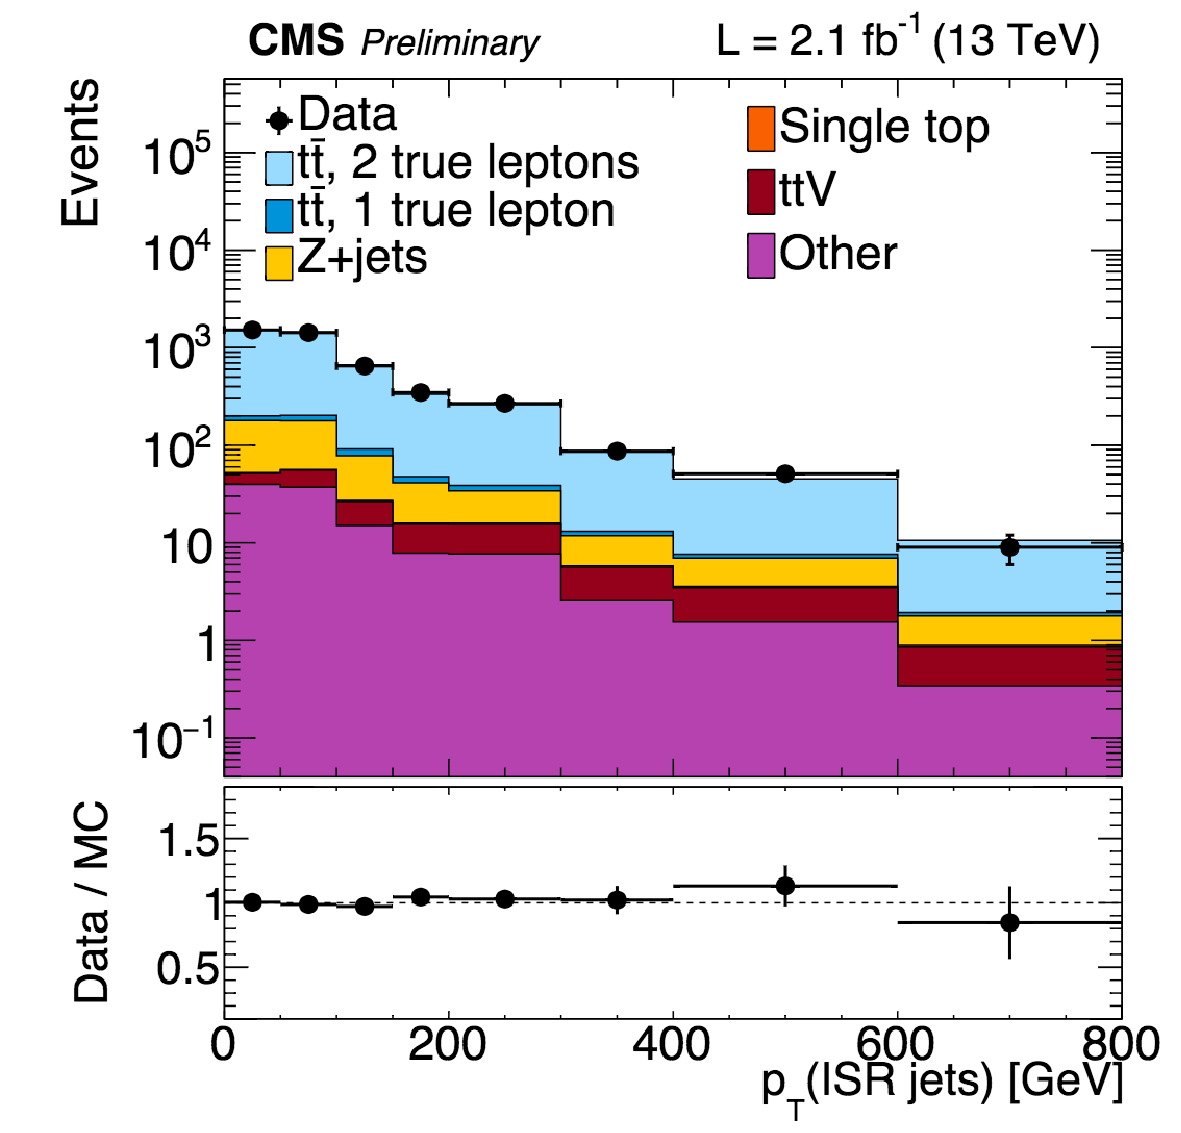
\includegraphics[width=0.4\textwidth]{results/figs/CMS-PAS-SUS-15-007_Figure_010-b.pdf} \\
\end{tabular}
\caption{
\label{fig:isrmodeling}
The ISR \pt\ in data and MC is shown for \zjets(left) and \ttbar(right).
}
\end{center}
\end{figure}

\clearpage

\section{Interpretation of the Results}
No significant excess is seen in any of the signal regions, so upper limits are set on the production cross section of a specific SUSY model.
The model used to interpret the results of this analysis is described in section~\ref{sec:signalmodel}.
This particular SUSY model is expected to have many jets, so most of the sensitivity comes from SRB.

The interpretation of these results is done by assigning 95\% confidence level upper limits according to the CLs technique~\cite{Read:2002hq}\cite{Junk:1999kv}.
These limits are obtained using the higgsCombine tool~\cite{ATL-PHYS-PUB-2011-011}.
The expected (observed) upper limit where this analysis is sensitive is for gluinos with mass up to 1.3 TeV when the neutralino mass is large,
and when the neutralino mass is small the expected (observed) upper limit is around 1.2 (1.1) TeV.
These results show a significant improvement over the 8 TeV result where we saw an observed and expected limit for gluino masses from 1 to 1.1 TeV.

\begin{figure}[!htb]
\begin{center}
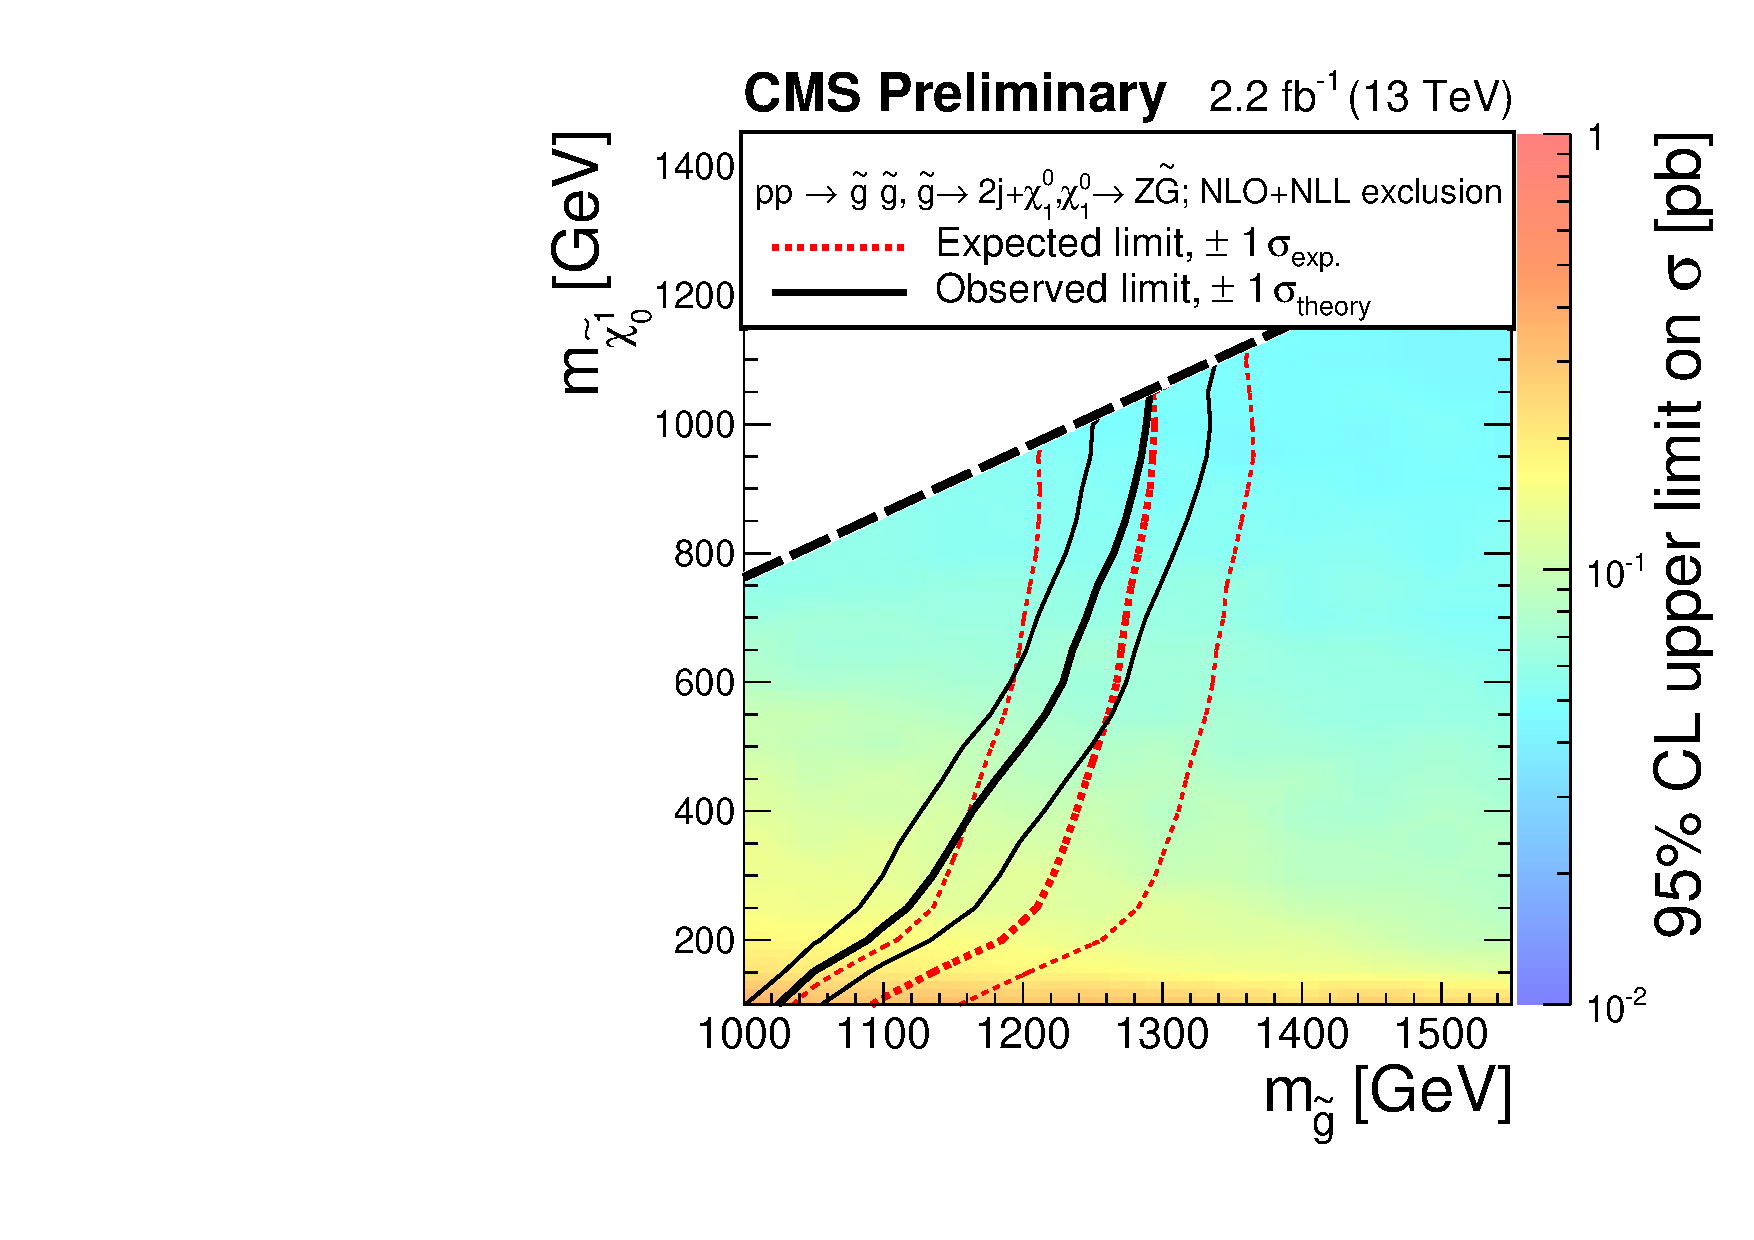
\includegraphics[width=0.8\textwidth]{results/figs/T5ZZ_Exclusion_13TeV.pdf}
\caption{
  Exclusion contours are shown when we interpret the results of this analysis in the SUSY model described in section~\ref{sec:signalmodel}.
  Everything to the left of the red (black) dotted line shows the masses which are exlcuded by the expected (observed) limit.
\label{fig:results_T5ZZ}}
\end{center}
\end{figure}


This is to acknowledge all the other members of the CMS experiment who made it possible to produce
the figures and tables appearing in this chapter.

\clearpage
